\documentclass[12pt, a4paper, oneside]{ctexbook}
\usepackage{amsmath, amsthm, amssymb, bm, graphicx, hyperref, mathrsfs}
\usepackage{geometry}
\usepackage{subfigure}
\usepackage{pdfpages}
\usepackage{hyperref}[colorlinks=true,linkcolor=black,citecolor=blue,urlcolor=blue]
\usepackage{listings, xcolor}
%设置引用格式
\hypersetup{
	colorlinks=true,linkcolor=black,colorlinks=true,linkcolor=black,citecolor=blue,urlcolor=blue
}
%在LateX中,参考文献的引用一般有两种方式,平 齐 时 用 命 令\cite{...}, 上 标 时用\textsuperscript{\cite{...}}

\CTEXsetup[format={\Large\bfseries}]{subsection}	%subsection 居左(默认居中)
\CTEXsetup[format={\huge\bfseries}]{section}	%section 居左(默认居中)


%代码配置
\lstset{
	breaklines,%自动换行
	columns=fixed,       
	numbers=none,                                        % 在左侧显示行号
	frame=none,		                                     % 不显示背景边框
	backgroundcolor=\color[RGB]{245,245,244},            % 设定背景颜色
	keywordstyle=\color[RGB]{40,40,255},                 % 设定关键字颜色
	numberstyle=\footnotesize\color{darkgray},           % 设定行号格式
	commentstyle=\it\color[RGB]{0,96,96},                % 设置代码注释的格式
	stringstyle=\rmfamily\slshape\color[RGB]{128,0,0},   % 设置字符串格式
	showstringspaces=false,                              % 不显示字符串中的空格
	language=C,                                          % 设置语言
	tabsize=2,
}

%配置纸张边缘
\geometry{left=2.54cm,right=2.54cm,top=3.18cm,bottom=3.18cm}


\title{{\Huge{\textbf{技术文档}}}\normalsize{\\——第六届全国大学生集成电路创新创业大赛景嘉微杯分赛区决赛提交文档}}
\author{队名:虹ヶ咲学园芯片设计同好会\\ 成员:黄金源\space邓立唯\space林明锋}
\date{\today}
\linespread{1.5}


\begin{document}
	
	\includepdf[page=1]{./pic/cover.pdf}
	
	%-----------------------封面------------------
	\maketitle	
	\pagenumbering{Roman}
	\setcounter{page}{1}
	%-----------------------前言------------------
	\begin{center}
		\Huge\textbf{前言}
	\end{center}~\
	
	本技术文档仅作为虹ヶ咲学园芯片设计同好会(成员:黄金源、邓立唯、林明锋)参加第六届全国大学生集成电路创新创业大赛景嘉微杯赛分赛区决赛提交文档供评委评分使用。
	~\\
	\begin{flushright}
		\includegraphics[width=0.25\linewidth]{pic/logo}\\
		\begin{tabular}{c}
			虹ヶ咲学园芯片设计同好会\\
			\today
		\end{tabular}
	\end{flushright}
	%-----------------------目录------------------
	\newpage
	\pagenumbering{Roman}	%Roman or arabic
	\setcounter{page}{1}
	\tableofcontents
	\newpage
	\setcounter{page}{1}
	\pagenumbering{arabic}
	
	%-----------------------正文----------------	
	\chapter{算法设计说明}
	\section{概要}
	\subsection{背景介绍}
	单幅图像超分辨率重建是指将一副低分辨率图像通过特定算法处理获得高分辨率图像的的一种技术。
	
	图像超分辨率重建一直以来都是图像处理领域中一个重要的研究方向之一,在医学、遥感、图像识别、网络媒体传输、动画制作与合成等领域都有着重要的应用。
	目前已有许多优秀的算法应用于现实的产品上,但是有效保持图像纹理细节且使图像边缘区域不失真,同时兼顾处理速度一直是图像超分辨率重建技术的一个难题。
	\par 在 GPU 处理领域,为了减轻像素引擎的负载,通常使用渲染低分辨率后经由算法放大至期望图像大小的方法已经成为一个被广泛使用的性能优化手段。
	实现一种对帧存颜色缓冲区图像的超采样处理 IP,用于硬件性能不足时将低分辨率图像放大至高分辨率,从而在尽可能贴合高分辨率渲染效果的同时提升帧率、降低功耗。
	\subsection{赛题分析}
	在本赛题中,由于举办方提供的图像样例仅包含像素信息,缺失了渲染相关的运动信息、位置信息、光线信息等,
	故可将本赛题视作 Single Image Super Resolution(SISR) 任务。由于比赛方限制使用基于神经网络设计的算法,
	我们队伍将基于传统算法结合机器学习的方法进行图像超分辨率核心算法设计。
	
	
	\section{算法分析}
	\subsection{下采样模型概括}
	在 SISR 任务中,实际上是完成了一个对低分辨率输入图像 LR 进行高分辨率图像 HR 的预测过程。图像的线性退化模型可以表示为式\ref{down_sample1}:
	\begin{equation}
		z=D_sHx + n \label{down_sample1}
	\end{equation}
	其中,$z$ 为输入大小为 $M*N$ 的 LR 图像;$x$ 为大小是 $Ms*Ns$ 的待预测 HR 图像;$H$ 是线性模糊核;$D_s$ 为下采样算子,系数 $s$ 是下采样的倍数; 
	$n$ 为额外的噪声。图像超分辨率的任务就是通过 $z$ 恢复出未知的 HR 图像 $x$。由于在退化模型之中,下采样操作会带来信息损失,
	同时随着下采样倍数 $s$ 增大,LR 所包含的 HR 信息越少。在这过程中,HR 与 LR 的对应是多对一的关系,完成超分辨率任务则变成了求解一个欠定逆问题,
	即求得结果可能产生多个输出。因此需要引入先验信息,通过约束获得唯一解。
	\par 在本次赛题中,由于给出的测试集为 GPU 渲染图片的 4 倍线性下采样图,公式 \ref{down_sample1} 中的线性模糊核 $H$ 则可以消去,
	同时假设没有引入来自其他的噪声干扰,则公式中噪声 $n$ 也可消去。最终得出得出式 \ref{down_sample2}
	\begin{equation}
		z=D_sx \label{down_sample2}
	\end{equation}
	
	\subsection{双三次插值算法介绍}
	在数值分析这个数学分支中,双三次插值(Bicubic)\textsuperscript{\cite{10}\cite{11}}是二维空间中最常用的插值算法,
	是三次插值的一个拓展。而在图像处理中,双三次插值算法更是首选。双三次插值需要参考周围 16 个像素($4 \times 4$)进行上采样,
	所得到的上采样图像会比最近邻插值和双线性插值更平滑,同时插值造成的伪影也更少。
	\begin{figure}[h]
		\centering
		\includegraphics[scale=0.8]{./pic/bicubic-introduction.pdf}
		\caption{双三次插值算法简介}
		\label{bicubic_introduction}
	\end{figure}
	\par
	作为一个整体,双三次插值算法需要计算插值像素中心与原始像素中心之间的距离。使用与距离存在映射关系的双三次插值函数计算相关系数,
	然后使用该系数与原始像素点相乘,最终与 16 个原始像素点的乘积之和就是新的插值像素点结果。
	可以简单地将新插值点看作与原始像素点对应的曼哈顿距离加权,可以用式 \ref{bicubic_1} 和式 \ref{bicubic_2} 表示:
	\begin{equation}
		SP_{\vec{s}}=\sum_{\vec{o}\in{RSB}}f_B(\vert\vec{s}-\vec{o}\vert)\cdot OP_{\vec{o}}		
		\label{bicubic_1}
	\end{equation}	
	
	\begin{equation}
		f_B(|x|)=
		\begin{cases}
			(\alpha + 2)|x|^3-(\alpha+3)|x|^2+1\quad &,if\ |x| \leq1\\
			\alpha|x|^3-5\alpha|x|^2+8\alpha|x|-4\alpha\quad&,if \ 1<|x|<2\\
			0&,otherwise				
			\label{bicubic_2}
		\end{cases}
	\end{equation}
	\par
	其中,$SP_{\vec{s}}$ 为插值后像素,$\vec{s}$ 是对应的索引向量。$RSB$ 为当前插值像素所在的插值块对应的原始像素的索引集合。
	$OP_{\vec{o}}$ 为原始像素,$\vec{o}$ 是对应的索引向量。$f_B$ 则是双三次插值的核心函数。
	\par 由于双三次插值算法在我们算法设计中为预处理部分,在实现上我们着重关注在硬件设计上,并针对性的进行了大量优化,
	具体请参考 \textbf{\nameref{appendix_a}} 介绍,此处不展开介绍。
	
	\subsection{高斯-拉普拉斯算子介绍}
	\subsubsection{概述}
	拉普拉斯算子是图像二阶空间导数的二维各向同性测度。图像的拉普拉斯算子强调快速强度变化的区域,因此经常用于边缘检测。
	拉普拉斯算子通常应用于近似高斯平滑滤波器进行平滑后的图像,以降低其对噪声的敏感性,因此这两种变体将在这里一起描述。
	该算子通常以单个灰度图像作为输入,生成另一个灰度图像作为输出。在本算法设计中,在该算子后引入一个阈值控制输出,从而实现图像二值化效果。
	\subsubsection{原理}
	记图片像素的强度值为$I(x,y)$ ,其所对应的拉普拉斯算子$L(x,y)$如式 \ref{lap} 所示:
	\begin{equation}	\label{lap}
		L(x,y)=\frac{\partial ^2 y}{\partial x^2} + \frac{\partial ^2 y}{\partial y^2}
	\end{equation}
	这个过程可以采用卷积核进行计算。由于图片是采用离散的像素值集合进行表示的,因此我们可以寻找一个近似于拉普拉斯算子的二阶导数离散卷积核。比如如下所示的两个卷积核:
	\begin{table}[h]
		\centering
		\begin{tabular}{lllll}
			\cline{1-3}
			\multicolumn{1}{|l|}{0}  & \multicolumn{1}{l|}{-1} & \multicolumn{1}{l|}{0}  &  &  \\ \cline{1-3}
			\multicolumn{1}{|l|}{-1} & \multicolumn{1}{l|}{4}  & \multicolumn{1}{l|}{-1} &  &  \\ \cline{1-3}
			\multicolumn{1}{|l|}{0}  & \multicolumn{1}{l|}{-1} & \multicolumn{1}{l|}{0}  &  &  \\ \cline{1-3}
			&                         &                         &  & 
		\end{tabular}
	\end{table}
	
	\begin{table}[h]
		\centering
		\begin{tabular}{lllll}
			\cline{1-3}
			\multicolumn{1}{|l|}{-1} & \multicolumn{1}{l|}{-1} & \multicolumn{1}{l|}{-1} &  &  \\ \cline{1-3}
			\multicolumn{1}{|l|}{-1} & \multicolumn{1}{l|}{8}  & \multicolumn{1}{l|}{-1} &  &  \\ \cline{1-3}
			\multicolumn{1}{|l|}{-1} & \multicolumn{1}{l|}{-1} & \multicolumn{1}{l|}{-1} &  &  \\ \cline{1-3}
			&                         &                         &  & 
		\end{tabular}
		\caption{近似于拉普拉斯算子的二阶导数离散卷积核}
	\end{table}
	以上的两个卷积核均可以近似为拉普拉斯算子。因为这两个卷积核都是对图片二阶导数的近似估计,它们对于图片中的噪声均很敏感。因此,为了解决这一问题,
	我们在进行拉普拉斯操作之前先对图像进行高斯平滑滤波处理,二维的高斯平滑卷积核可以用式 \ref{gauss} 进行表示。
	\begin{equation}	\label{gauss}
		G_\sigma (x,y)=\frac{1}{2\pi \sigma ^2} exp(-\frac{x^2+y^2}{2\sigma ^2}) 
	\end{equation}
	先利用高斯平滑滤波进行处理,可以降低图片中的高频噪声,方便后续的拉普拉斯操作。
	
	\subsection{局部二值模式介绍}
	\subsubsection{概述}
	局部二值模式 (LBP, Local Binary Pattern)\textsuperscript{\cite{8}}\textsuperscript{\cite{9}}\textsuperscript{\cite{13}} 是一种用来描述图像局部纹理特征的算子;
	它具有旋转不变形和灰度不变性等显著优点,适合用来提取图像的局部纹理特征。	
	\subsubsection{原理}
	原始的 LBP 算子\textsuperscript{\cite{13}}定义在 $3\times3$ 的窗口内,以窗口中心像素为阈值,将相邻的 8 个像素的灰度值与其进行比较,若周围像素值大于中心像素值,
	则该像素点的位置被标记为 1,否则为 0。如此,$3\times3$ 领域内的 8 个点经过比较可产生 8 位二进制数 (通常转换为十进制数即 LBP 码,共 256 种),即得到该窗口中心像素点的 LBP 值,
	并用这个值来反映该区域的纹理信息。可用公式 \ref{lbp} 来进行描述该过程。
	\begin{equation}
		LBP_{P,R}=\sum_{p=0}^{P-1}s(g_p-g_c)2^{p},\quad s(x)=\begin{cases}
			1  &,x\geq0\\
			0  &,x\le0 
		\end{cases}
		\label{lbp}
	\end{equation}
	\par
	实际上,基于原始 LBP 算子的纹理分类方法过于粗糙,对于图像区域的纹理分类有一定的局限性。
	后来出现了不少基于 LBP 改进的算法,通过引入新的参数,来获得更好的纹理分类能力。
	如圆形 LBP 算子\textsuperscript{\cite{8}}具有旋转不变性、经过统一编码 (Uniform Pattern) 后对算子种类进行降维,
	CLBP 算子\textsuperscript{\cite{9}}引入图像的局部梯度参数以增强纹理分类能力。
	\subsection{RAISR 算法}
	\subsubsection{概述}
	Google 在 2016 年提出了 \textbf{RAISR}\textsuperscript{\cite{1}} 算法,一种基于样本学习的超分辨率算法。 
	RAISR 主要的特点是快速、准确,在运行速度上比基于深度学习的方法有大幅提升,同时保持了具有竞争力的图像重建质量。
	其核心思想是通过简单的插值方式把 LR 图像转化成 Pre-HR 图像,然后根据 Pre-HR 图像局部的梯度信息来对图像块进行分类,
	对于不同类别的图像块对应采用不同的与训练的滤波器进行卷积操作对图像纹理进行增强。
	在足够的训练数据下,通过学习一组滤波器建立成对的 LR patch与 HR 像素的映射关系。
	\par RAISR 将 patch 分为了 216 类并结合 $R^2$ 个像素类型 (R为上采样因子),这其中包括了 3类像素强度、24类纹理角度、3类图像块相关性。
	因此,当上采样因子 $R$ 为4时,便需要 3456 个大小为 11 x 11 的滤波器。
	通过哈希映射的方式将 patch 分类到不同类别中,而不需要使用较为复杂的聚类方式如 K-means\textsuperscript{\cite{2}}、或者是高斯混合模型\textsuperscript{\cite{3}},
	从而降低分类查找时间。在 RAISR 中,哈希表键值是通过计算 patch 的局部梯度统计来获得。接下来我们会分析 RAISR 的一些具体实现。
	\subsubsection{哈希表键计算方法}
	通过特征分析\textsuperscript{\cite{6}}来计算用作哈希表键的图像块的局部梯度特征。第 $k$ 个的最近领域通常是一个 $\sqrt{n}*\sqrt{n}$ 的 patch,其中,像素包含于 $k_1,...,k_n$。
	每个图像块的局部梯度特征放置在一个 $n \times 2$ 的矩阵 \ref{matrix_1} 中:
	\begin{equation}
		G_k=
		\left[
		\begin{matrix}
			{g_{x_{k_1}}} & {g_{y_{k_1}}}\\
			\vdots & \vdots\\
			{g_{x_{k_n}}} & {g_{y_{k_n}}}
		\end{matrix}
		\right]\label{matrix_1}
	\end{equation}
	\par 在特征分析\textsuperscript{\cite{6}}中,局部梯度特征可以通过奇异值分解 (SVD) 进行计算。求解出来的右向量表示为该图像块的梯度方向,
	两个奇异值用于表示梯度的强度和相关性。通过一个可分离的归一化高斯核构建了一个对角矩阵 $W_k$,用于简化特征值分解。
	根据 $G_k^TW_kG_k$ 矩阵的特征分解得到较大的特征值 $\lambda_1^k$ 、较小的特征值 $\lambda_2^k$ 和两个特征向量 $\phi_1^k$ 和 $\phi_2^k$,
	用来表示梯度的强度 $\lambda_k$、角度 $\theta_k$ 和相关系数 $\mu_k$,其中
	\begin{equation}
		\lambda_k=\lambda_1^k
	\end{equation}
	\begin{equation}
		\theta_k=\arctan(\frac{\phi_{1,y}^k}{\phi_{1,x}^k}) 
	\end{equation}
	\begin{equation}
		\mu_k=\frac{\sqrt{\lambda_1^k}-\sqrt{\lambda_2^k}}{\sqrt{\lambda_1^k}+\sqrt{\lambda_2^k}} 
	\end{equation}
	这三个哈希表键量化后可以用 $\lambda$,$\theta$, $\mu$ 来表示,其中
	\begin{equation}
		\lambda=\lceil\frac{\lambda_k}{Q_s}\rceil		\label{hash_7}
	\end{equation}
	\begin{equation}
		\theta=\lceil\frac{\theta_k}{Q_\theta}\rceil	\label{hash_8}
	\end{equation}
	\begin{equation}
		\mu=\lceil\frac{\mu_k}{Q_\mu}\rceil				\label{hash_9}
	\end{equation}
	在以上式 \ref{hash_7} 、式 \ref{hash_8} 和式 \ref{hash_9} 中,$Q_s$、$Q_\theta$、$Q_\mu$ 分别代表了强度、角度和相关系数的量化因子。
	通过这三种参数,构建了 216 个哈希键映射分类。
	
	\subsubsection{滤波器学习}
	在 RAISR 的学习阶段,需要通过建立一个 LR 图像块与 HR 像素点映射的训练数据集,用于学习一个 $d\times d$ 的滤波器 $h$。
	滤波器可以通用求解最小二乘法最小值来计算:
	\begin{equation}
		h=\min_h\sum_{i=1}^L\lVert{A_ih-b_i}\rVert_2^2 \label{filter_10}
	\end{equation} 
	其中,$h$ 是一个 $d^2 \times 1$ 向量表示学习的滤波器,$A_i$ 是由 Pre-SR 图像 $y_i$ 中提取图像块 $d\times d$ 后组成的大小为 $MN\times d^2$ 矩阵,
	$b_i$ 是由 HR 图像 $x_i$ 中提取的像素点所构成,对应 $y_i$ 图像块的中心坐标。
	在论文\textsuperscript{\cite{1}}中,作者为了降低求解滤波器的运算量和数据存储,将式\ref{filter_10}拓展为:
	\begin{equation}
		h=\min_h\lVert Qh-V\rVert_2^2		\label{filter_11}
	\end{equation}
	其中 $Q=A^TA$,$V=A^Tb$。经过这样的转换可以降低数据存储空间以及求解时候的运算,可以表示为:
	\begin{equation}
		Q=A^TA=\sum_{i=1}^LA_i^TA_i
	\end{equation}
	\begin{equation}
		V=A^Tb=\sum_{i=1}^LA_i^Tb_i
	\end{equation}
	其中,$Q$ 是一个 $d^2 \times d^2$ 的小矩阵和 $V$ 是一个 $d^2 \times 1$ 的列向量。到此滤波器的学习介绍就此结束。
	
	\subsubsection{CT变换}
	由于在学习滤波器的时候会引入锐化操作,在使用该滤波器应用于简易插值后的图像,可能会引起结构变形。为了保留重要的结构,作者引入了 CT变换\textsuperscript{\cite{7}},作用于简易插值后的图像与滤波后的图像。
	具体变换如图 \ref{CT_tran} 所示:
	\begin{figure}[h]
		\centering
		\includegraphics[scale=0.88]{./pic/CT.pdf}
		\caption{CT变换}
		\label{CT_tran}
	\end{figure}
	通过一个 $3\times 3$ 的图像块的周围像素与中心像素构建出一个布尔类型进行比较,然后以汉明距离来计算每个像素的变化位数。
	由于结构的变化是取决于汉明距离的,可以根据变化的位数来确定权重用于加权插值图像与滤波图像,从而得到输出图像。至此,RAISR 的核心设计思路已经清晰。
	
	\section{算法优化}
	通过上节我们可以看到,RAISR 作者对于滤波器的学习以及应用进行了不少的优化,但是对于我们将该算法应用到硬件实现上,有着不小的挑战。第一个是在于,每个像素类型需要学习 216 个滤波器,
	而对于进行 4 倍上采样的整幅图像可分为 16 种类型,总共就需要 3456 个滤波器进行片上存储。在 FPGA 上存储如此大量的数据是不划算的。
	第二点是,为了能获得像素更多的信息,RAISR 采用了 $11\times11$ 大小的滤波器进行卷积,这对于硬件资源消耗量极大,
	在考虑量化同时保留运算过程中数据合适位宽并满足运算时延,每个像素进行锐化操作至少需要 180 个 DSP 进行乘累加运算(不考虑硬件复用以减少资源消耗),总延时至少 12 个时钟周期输出延迟,该结果已经考虑了使用树形结构对数据进行运算。
	第三点,哈希表键的运算不仅需要进行除法、开方及反正切运算,还需要进行奇异值分解,这对于 FPGA 实时性设计要求难度提升了一个等级。
	\subsection{概述}
	我们提出了一个创新的 \textbf{LBP-RAISR} 算法,以 \textbf{RAISR} 为主体框架,整体上分为了三个阶段。
	第一步,通过双三次插值算法\textsuperscript{\cite{4}\cite{5}},将 LR 图像映射到 HR 图像上,得到最终需要的目的分辨率图像 Pre-SR;
	第二步,对图像以每个像素为中心进行 $5\times5$ 分块,遍历 Pre-HR 图像的每一个图像块,
	进行高斯-拉普拉斯(LoG)纹理检测后使用 CLBP 算法\textsuperscript{\cite{8}\cite{9}}结合角度信息求解进行纹理分类。
	显而易见,这里我们的设计与 \textbf{RAISR} 有较大的区别,这是出于对硬件设计的考量,具体的设计细节会在下一节和 RTL设计文档 中详细解释。
	第三步,利用上一步的得到每个图像块的类型找到对应的滤波器,作用于图像块进行卷积,得到更接近于原始 HR 的像素,最后得到更高质量的 SR 图像。
	整体框架如图\ref{overview}所示。
	\begin{figure}[h]
		\centering
		\includegraphics[scale=0.65]{./pic/overview.pdf}
		\caption{算法架构}
		\label{overview}
	\end{figure}
	\subsection{实现步骤}
	\subsubsection{双三次插值}
	作为第一步,我们需要将 LR 图像先上采样到需要的分辨率,可以使用传统的插值方法如最近邻插值、双线性插值、双三次插值、Lanczos 插值等算法。
	由于考虑到上采样图片的质量效果会应影响到最终的高分辨率图片质量与运算过程中的尽可能降低复杂度,双三次插值成为了我们算法预处理的最优选择。
	\subsubsection{纹理分类}
	我们对经过 4 倍上采样后的 Pre-SR 图片先进行高斯-拉普拉斯滤波(LoG)\textsuperscript{\cite{12}},然后给定一个阈值区间对进行滤波后的像素值进行二值化操作,
	采用 CLBP 算法对二值化后的图像纹理进行按块分类。这里需要注意的是,我们采用 $5 \times 5$ 的图像块进行纹理分类,由于已经对图像块进行了纹理检测这一步操作,
	所以 CLBP 算法步骤我们并没有严格执行,保留 $C$ 中心像素与 $u$ 统一编码这两个参数。考虑到该算法需要对圆形区域检测需要进行三角函数进行运算,
	我们将其近似等效为最外边缘的二值像素,从而减轻运算量。但是 CLBP 算法经过统一编码后具有旋转不变形,与滤波器需要学习局部纹理方向角度特征相矛盾,
	故此我们增加了一步操作,当进行对像素统一编码时,保留了角度信息,从而增加选择滤波器参数条件。此时,纹理分类结束。
	\subsubsection{卷积输出}
	在上一步中我们已经通过纹理分类得到了图像块的纹理类型,根据这个类型我们可以选择预学习的滤波器,对相应的 Pre-SR 图像块进行卷积操作,从而得到了 SR 像素,最终输出 SR 图像。
	
	\section{效果展示}
	我们将提出的算法与 RAISR 进行了对比,	其中 Set5 是单帧图像超分辨率任务中最常用的数据集,GameSet 是景嘉微在本次杯赛中提供的测试效果图片。
	
	\begin{figure}[h]
		\centering
		\subfigure[GT]{
			\includegraphics[scale=0.35]{./pic/GT-1.png}
		}
		\quad
		\subfigure[bicubic]{
			\includegraphics[scale=0.35]{./pic/bicubic-1.png}
		}
		\quad
		\subfigure[raisr]{
			\includegraphics[scale=0.35]{./pic/raisr-1.png}
		}
		\quad
		\subfigure[lbp-raisr]{
			\includegraphics[scale=0.35]{./pic/lbp-raisr-1.png}
		}
		\caption{各算法实现效果对比-例1}
	\end{figure}
	
	\begin{figure}[h]
		\centering
		\subfigure[GT]{
			\includegraphics[scale=0.7]{./pic/GT-2.png}
		}
		\quad
		\subfigure[bicubic]{
			\includegraphics[scale=0.7]{./pic/bicubic-2.png}
		}
		\quad
		\subfigure[raisr]{
			\includegraphics[scale=0.7]{./pic/raisr-2.png}
		}
		\quad
		\subfigure[lbp-raisr]{
			\includegraphics[scale=0.7]{./pic/lbp-raisr-2.png}
		}
		\caption{各算法实现效果对比-例2}
	\end{figure}
	
	
	%	\newcounter{Rownumber}
	%	\newcommand{\Rown}{\stepcounter{Rownumber}\theRownumber}
	\begin{table}[htb]
		\small
		\begin{tabular}{|c|c|c|c|c|c|c|}
			\hline
			\textbf{DataSet} & \textbf{Scale} & \textbf{Bilinear} & \textbf{Bicubic} & \textbf{RAISR} & \textbf{LBP-RAISR} & \textbf{\begin{tabular}[c]{@{}c@{}}LBP-RAISR\\ (Quantized)\end{tabular}} \\ \hline
			Set5(PSNR)       & x4             & 25.79             & 26.84            & 27.05          & \textbf{27.61}     & \textbf{27.61}\\ \hline
			Set5(SSIM)       & x4             & 0.765             & 0.790            & 0.803          & 0.812     			& \textbf{0.817}                                                                    \\ \hline
			Set5(LPIPS)      & x4             & 0.335             & 0.310            & 0.269          & \textbf{0.198}     & 0.200                                                                    \\ \hline
			GameSet(PSNR)    & x4             & 30.83             & 31.51            & 31.59          & \textbf{32.02}     & 32.00                                                                    \\ \hline
			GameSet(SSIM)    & x4             & 0.847             & 0.862            & 0.861          & 0.870     		& \textbf{0.871}                                                                    \\ \hline
			GameSet(LPIPS)   & x4             & 0.288             & 0.265            & 0.263          & \textbf{0.209}     & 0.211                                                                    \\ \hline
		\end{tabular}
		\caption{各算法实现评分对比}
	\end{table}
	
	\section{总结}
	基于 RASIR\textsuperscript{\cite{1}} 的整体思路,我们提出了改进的 LBP-RAISR 算法。LBP-RAISR 背后的核心思想与 RAISR 相同,
	学习从低分辨率图像到高分辨率图像的映射关系,用于增强经过简单插值后的图像质量。锐化过程是通过使用一组滤波器,对简单插值放大的 Pre-SR 图像进行操作。
	这些滤波器旨在最小化输入图像和真实图像之间的欧氏距离。更具体地说,LBP-RAISR 使用了一种更简便快捷的纹理分类方法,从存储空间上和运算量上做了大量的优化,
	同时也保留了图像质量的效果。根据大量实验得知,可以较好的提升 RAISR 的性能以及运算时间。
	经过量化后适配硬件设计并没有损失太大的图像质量。由于我们采用的是基于中心的局部二值模式 (CLBP) 变体与高斯-拉普拉斯滤波 (LoG) 结合的算法进行纹理分类,与 RAISR 中的哈希映射方法相比较,进一步减少了运算量,
	同时选择滤波器的方法是固定的,这对于硬件上实现是高效便捷的。从更广泛的角度来看,我们希望 LBP-RAISR 中预学习的滤波器映射与训练集的关联影响尽可能小,
	在这种情况下,学习的过滤器可以用于任意尺寸输入图像进行 $\times4$ 的超分辨率图像输出。
	由于运算量的大大降低,让高分辨率图像进行实时的超分辨率任务也是可能的。在软件实现过程中,多线程优化下处理一张 4K 图像仅需要 3.6 秒左右(包含图像读写时间)。
	
	
	
		
		%-----------------------正文----------------	
	\chapter{实现函数说明}
		\section{基本介绍}
		\subsection{整体流程}
		\begin{figure}[h]
			\centering
			\includegraphics[scale=0.5]{pic/overview}
			\caption{程序整体流程}
			\label{fig:overview}
		\end{figure}
		\subsection{数据结构}
		\subsubsection{图片格式}
		\begin{enumerate}
			\item \textbf{BitmapHead:}包含bmp文件信息头各个信息相对于文件头的偏移量
			\begin{lstlisting}
typedef struct {
	uint32_t biSize;
	uint32_t biWidth;
	uint32_t biHeight;
	uint16_t biPlanes;
	uint16_t biBitCount;
	uint32_t biCompression;
	uint32_t biSizeImage;
	uint32_t biXPelsPerMeter;
	uint32_t biYPelsPerMeter;
	uint32_t biClrUsed;
	uint32_t biClrImportant;
}BitmapHead;
			\end{lstlisting}
			
			
			\item \textbf{Bitmap:}包含bmp图像的文件信息:文件名、文件信息头结构体指针和图像数据指针
			\begin{lstlisting}
typedef struct {
	char* fileName;
	BitmapHead *head;
	ImageMat *image;
}Bitmap;
			\end{lstlisting}
			
			
			\item \textbf{ImageMat:} 包含图像的宽度、高度和数据所在的内存首地址
			\begin{lstlisting}[numbers=none]
typedef struct {
	int width;
	int height;
	uint8_t *pData;
}ImageMat;		
			\end{lstlisting}			
		\end{enumerate}
		
		\subsubsection{量化}
		\begin{enumerate}
			\item \textbf{qint16\_t:}带量化位数的16位变量类型,real表示变量真实值,Qn表示该变量需要量化的位数
			\begin{lstlisting}
typedef struct {
	int16_t real;		
	uint8_t Qn;			
}qint16_t;					
			\end{lstlisting}
			\item \textbf{qint32\_t:}带量化位数的32位变量类型,real表示变量真实值,Qn表示该变量需要量化的位数
			\begin{lstlisting}
typedef struct {
	int32_t real;	
	uint8_t Qn;		
}qint32_t;				
			\end{lstlisting}
			\item \textbf{qImageMat:}带量化位数的图像数据存储格式
			\begin{lstlisting}
typedef struct {
	int width;
	int height;
	qint16_t* pData;
}qImageMat;			
			\end{lstlisting}
			\item \textbf{QuantizeError:}量化运算成功或失败标志
			\begin{lstlisting}
typedef enum {
	OK = 0,
	QN_ALARGE,
	QN_BLARGE
}QuantizeError;		
			\end{lstlisting}
			\item \textbf{qCompareRes:}量化比较结果
			\begin{lstlisting}
typedef enum {
	Q_EQ = 0,	
	Q_GR,     // >
	Q_LT      // <
}qCompareRes;		
			\end{lstlisting}
			
		\end{enumerate}
		
		
		
		
		
		
		\section{实现函数细节}	
		%%--------------------双三----------------	
		\subsection{超分辨率实现}
		\begin{enumerate}
			\item \textbf{双三次插值}
			\begin{lstlisting}[numbers=none]
				void bicubic_interp_fixed(Bitmap* bitmap, Bitmap** pOutput);
			\end{lstlisting}
			\textbf{参数:} \par bitmap: 要进行双三次插值的图像 \par pBitmap: Bitmap类型的指针变量,用于存储fileName的文件信息 \\
			\textbf{返回值:}\par 无返回值\\
			\textbf{作用:}\par 对输入图像进行双三次插值,提高图像分辨率\\
			双三次插值内部实现具体可参考 \textbf{\nameref{appendix_a}}。
			
			\item \textbf{上采样——单通道实现}
			\begin{lstlisting}[numbers=none]
void upsampling(ImageMat* src, ImageMat** dst, qint16_t** weight, uint32_t num_instance);			
			\end{lstlisting}
			\textbf{参数:} \par src: 要进行质量增强的图像 \par dst: 质量增强后的图像\par weight: 带有量化位数的权重\par num\_instance: 需要运行的线程数
			\textbf{返回值:}\par 无返回值\\
			\textbf{作用:}\par 对输入图像进行纹理分类并进行锐化操作,提高图像质量\\
			\textbf{说明:}\par 在本次设计中,需要先根据patch\_edge进行图像分类,再将图像的patch 和 patch\_edge 一一对应,执行相应计算。本次设计中,需要处理 4k 分辨率图像,采用顺序执行的方式非常耗费时间,因此该函数采用了并行计算的方式,先将待处理图像分为 num\_instance 个部分,每个部分创建一个对应的线程进行并行计算,等待所有线程返回后再执行下一步计算,大大提高了运行速率。
			
			\item \textbf{上采样——RGB通道实现}
			\begin{lstlisting}[numbers=none]
void upsampling_rgb(ImageMat* src, ImageMat** dst, qint16_t** weight, uint32_t num_instance, ImageMat* src_r, ImageMat* src_g, ImageMat* src_b, ImageMat** dst_r, ImageMat** dst_g, ImageMat** dst_b);
			\end{lstlisting}
			
			\textbf{参数:} \par src: 要进行纹理分类的灰度图像 \par dst: 质量增强后的图像\par weight: 带有量化位数的权重\par num\_instance: 需要运行的线程数 \\ src\_r: 需要进行质量提升的R通道图像 \\ src\_g: 需要进行质量提升的G通道图像 \\ src\_b: 需要进行质量提升的B通道图像 \\ dst\_r: 质量增强后的R通道图像 \\ dst\_g: 质量增强后的G通道图像 \\ dst\_b: 质量增强后的B通道图像\\
			\textbf{返回值:}\par 无返回值\\
			\textbf{作用:}\par 对输入图像进行纹理分类并进行锐化操作,提高图像质量\\
			\textbf{说明:}\par 该函数与上一函数不同,对三个通道同时继续了锐化操作,进而获得更好的整体图像质量。
			
			
		\end{enumerate}
		
		
		
		%%--------------------锐化----------------	
		\subsection{锐化}
		%%--------------------其余组件----------------	
		\subsection{其余组件}
		\subsubsection{内存管理}
		\begin{lstlisting}[numbers=none]
void freeqWeightSpace(qint16_t ** weight, int32_t type);
		\end{lstlisting}
		\textbf{参数:} \par weight : qint\_16 类型的指针 \par type: int32\_t 类型的变量 \\
		\textbf{返回值:}\par 无返回值 \\
		\textbf{作用:}\par 用于释放申请的内容空间\\
		
		
		\subsubsection{图片读取与格式转换}
		图片处理接口细节可参考 \textbf{\nameref{appendix_a}}。
		\begin{enumerate}
			\item \textbf{ReadBitmap}——读取bmp格式图片
			\begin{lstlisting}[numbers=none]
BitmapReadError ReadBitmap(const char* fileName, Bitmap** pBitmap);
			\end{lstlisting}
			\textbf{参数:} \par fileName: 要读取的bmp格式图片路径 \par pBitmap: Bitmap类型的指针变量,用于存储fileName的文件信息 \\
			\textbf{返回值:}\par BitmapReadError 类型的枚举变量,用于表示读取文件是否成功\\
			\textbf{作用:}\par 用于读取bmp格式图片\\
			
			\item \textbf{WriteBitmap}——写bmp格式图片
			\begin{lstlisting}[numbers=none]
BitmapWriteError WriteBitmap(Bitmap* bitmap, const char* fileName);
			\end{lstlisting}
			\textbf{参数:} \par fileName: 要写入的bmp格式图像路径 \par bitmap: Bitmap类型的指针变量,用于存储fileName的文件信息 \\
			\textbf{返回值:}\par BitmapWriteError 类型的枚举变量,用于表示写入文件是否成功\\
			\textbf{作用:}\par 用于写bmp格式图像\\
			
			\item \textbf{ImageMatRGBtoYUV}——将RGB编码图片转换为YUV编码图片
			\begin{lstlisting}[numbers=none]
void ImageMatRGBtoYUV(ImageMat* mat);
			\end{lstlisting}
			\textbf{参数:} \par mat: ImageMat类型的结构体指针,用于存储图像的长度、宽度和数据信息\par 
			\textbf{返回值:}\par 无返回值 \\
			\textbf{作用:}\par  将RGB编码图片转换为YUV编码图像\\
			
			\item \textbf{ImageMatYUVtoRGB}——将YUV编码图片转换为RGB编码图片
			\begin{lstlisting}[numbers=none]
void ImageMatYUVtoRGB(ImageMat* mat);
			\end{lstlisting}
			\textbf{参数:} \par mat: ImageMat类型的结构体指针,用于存储图像的长度、宽度和数据信息\par 
			\textbf{返回值:}\par 无返回值 \\
			\textbf{作用:}\par  将YUV编码图像转换为RGB编码图像\\
			\item \textbf{qImageMatRGBtoYUV}——将量化的RGB编码图片转换为YUV编码图片
			\begin{lstlisting}[numbers=none]
void qImageMatRGBtoYUV(qImageMat* qmat_r, qImageMat* qmat_g, qImageMat* qmat_b, qImageMat* qmat_y, qImageMat* qmat_u, qImageMat* qmat_v);
			\end{lstlisting}
			\textbf{参数:} \\
			qmat\_r: qImageMat类型的结构体指针,用于存储量化图像R通道的长度、宽度和数据信息 \\ 
			qmat\_g: qImageMat类型的结构体指针,用于存储量化图像G通道的长度、宽度和数据信息 \\ 
			qmat\_b: qImageMat类型的结构体指针,用于存储量化图像B通道的长度、宽度和数据信息 \\ 
			qmat\_y: qImageMat类型的结构体指针,用于存储量化图像Y通道的长度、宽度和数据信息 \\ 
			qmat\_u: qImageMat类型的结构体指针,用于存储量化图像U通道的长度、宽度和数据信息 \\
			qmat\_v: qImageMat类型的结构体指针,用于存储量化图像V通道的长度、宽度和数据信息 \\
			\textbf{返回值:} \\ 无返回值 \\
			\textbf{作用:} \\ 将量化的RGB编码图片转换为量化的YUV编码图像
			
			\item \textbf{qImageMatYUVtoRGB}——将量化的YUV编码图片转换为RGB编码图片
			\begin{lstlisting}
void qImageMatYUVtoRGB(qImageMat* qmat_y, qImageMat* qmat_u, qImageMat* qmat_v, qImageMat* qmat_r, qImageMat* qmat_g, qImageMat* qmat_b);
			\end{lstlisting}
			\textbf{参数:} \\
			qmat\_y: qImageMat类型的结构体指针,用于存储量化图像Y通道的长度、宽度和数据信息 \\ 
			qmat\_u: qImageMat类型的结构体指针,用于存储量化图像U通道的长度、宽度和数据信息 \\
			qmat\_v: qImageMat类型的结构体指针,用于存储量化图像V通道的长度、宽度和数据信息 \\
			qmat\_r: qImageMat类型的结构体指针,用于存储量化图像R通道的长度、宽度和数据信息 \\ 
			qmat\_g: qImageMat类型的结构体指针,用于存储量化图像G通道的长度、宽度和数据信息 \\ 
			qmat\_b: qImageMat类型的结构体指针,用于存储量化图像B通道的长度、宽度和数据信息 \\ 
			\textbf{返回值:} \\ 无返回值 \\
			\textbf{作用:} \\ 将量化的YUV编码图片转换为量化的RGB编码图像
			
			
			\item \textbf{ImageMatRGBtoYUV}——提取YUV编码格式中Y通道数据
			\begin{lstlisting}[numbers=none]
ImageMat* splitYChannel(ImageMat* mat);
			\end{lstlisting}
			\textbf{参数:} \par mat: ImageMat类型的结构体指针,用于存储图像的长度、宽度和数据信息\par 
			\textbf{返回值:}\par ImageMat 类型指针,存储图片的长度、宽度和YUV编码格式中Y通道数据 \\
			\textbf{作用:}\par 提取YUV编码格式中Y通道数据 \\
			
			\item \textbf{mergeYChannel2Image}——将YUV编码格式中Y通道数据合并到图像中
			\begin{lstlisting}[numbers=none]
void mergeYChannel2Image(ImageMat* img, ImageMat* im_y);
			\end{lstlisting}
			\textbf{参数:} \par mat: 要合并的目标图像,ImageMat类型的结构体指针,用于存储图像的长度、宽度和数据信息\par im\_y:ImageMat 类型指针,存储要合并图像的长度、宽度和Y通道数据信息 \\
			\textbf{返回值:}\par 无返回值 \\
			\textbf{作用:}\par 将YUV编码格式中Y通道数据合并到图像中 \\			
			
			\item \textbf{DestoryImageMat}——释放图像内存空间
			\begin{lstlisting}[numbers=none]
void DestoryImageMat(ImageMat* mat);
			\end{lstlisting}
			\textbf{参数:} \par mat: ImageMat 类型的结构体指针,用于存储图像的长度、宽度和数据信息\par 
			\textbf{返回值:}\par 无返回值 \\
			\textbf{作用:}\par 内部调用 free 释放申请的图像内存 \\					
		\end{enumerate}

		\chapter{寄存器说明}
		\newpage
		\begin{center}
			本 IP 有计划使用寄存器文件进行参数权重配置,\\
			已留有 Dummy 接口用于与 SoC 的 AXI-4 Full 接口互联。\\
			\textbf{该文档会在下一大版本中进行更新 : )}
		\end{center}
	
	\chapter{RTL模块设计说明}
	%-----------------------正文----------------	
	\section{概要}
	上采样 IP 设计采用了模块化设计,主要分为四大部分:
	\begin{enumerate}
		\item Bicubic 上采样模块
		\item 纹理分类模块
		\item 自适应锐化模块
		\item 色域转换模块
	\end{enumerate}
	
	\begin{figure}[h]
		\centering
		\includegraphics[scale=0.4]{pic/all.drawio.pdf}
		\caption{IP 概览}
		\label{fig:ip-overview}
	\end{figure}
	
	\section{上采样模块}
	具体说明详见 \textbf{\nameref{appendix_a}}。
	
	\section{纹理分类模块}
	纹理分类 IP 可提供对于单通道图像每个 $5\times5$ 或 $3\times3$ 图像块的纹理特征进行实时分类。
	包含了一个归一化高斯卷积核、一个标准拉普拉斯算子、一个 LBP 分类器、三个行缓冲模块、
	一个滤波器参数存储单元和一个控制单元。
	为了确保卷积操作后图像仍保持原始尺寸,行缓冲模块包含了图像填充处理操作与数据映射模块,由控制单元进行管理。
	
	\begin{figure}[h]
		\centering
		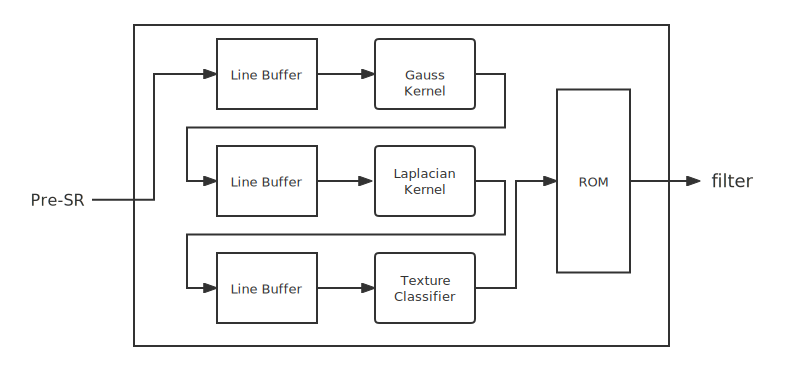
\includegraphics[scale=0.55]{./pic/texture}
		\caption{纹理分类模块结构图}
		\label{fig:texture}
	\end{figure}
	
	
	
	\subsection{运算位宽与量化}
	为了节省片上资源的消耗,最大化提升 DSP 利用率,在本模块中,不同部分对于 DSP48E2 均有不同程度上的优化。
	其中,针对高斯滤波卷积,将核内权重进行 9 位无符号量化,在保证高斯卷积核性能的同时充分利用了 DSP48E2 
	单元的乘法器。这种量化方法仅支持 8 位图像输入。另外,为了保证后续拉普拉斯滤波数据误差尽可能降低,
	我们将高斯滤波后的数据量化为 20 位,尽可能保留数据位宽,避免引入过大误差影响后续操作。
	在完成拉普拉斯算子卷积后生成的是 1 位图像输出至 LBP 分类器。
	\subsection{高斯卷积核}
	高斯卷积核包含了一个高斯系数寄存器单元、一组并行乘法器单元、一组并行的加法器单元和一组并行舍入单元。
	\begin{figure}[h]
		\centering
		\includegraphics[scale=0.55]{pic/gaussian_filter}
		\caption{高斯卷积核结构图}
		\label{fig:gaussianfilter}
	\end{figure}
	每个像素进行高斯滤波卷积是以像素本身为中心,边缘 $5\times5$ 的像素块作为数据输入。
	每个像素块需要与对应的高斯系数进行相乘然后累和。该高斯卷积核 IP 每个时钟周期处理 4 个像素。
	\subsubsection{高斯系数寄存器单元}
	高斯滤波卷积核系数是由 $\sigma$ 所决定,在运行过程中,$\sigma$ 不会发生改变,所以该系数为常数。
	同时,$5\times5$ 卷积核系数与所在卷积核的位置有关,并意义对应,因此25 个系数只需要存储 6 个系数即可,其余均可通过对称性获取。
	\begin{figure}[h]
		\centering
		\includegraphics[scale=0.4]{pic/number}
		\caption{高斯卷积核数据矩阵数据分布}
		\label{fig:number}
	\end{figure}
	\subsubsection{乘法器单元} \label{mul_unit}
	并行乘法单元包含了 7 个 DSP48E2 用于实现 $5\times5$ 大小的卷积乘法操作。
	在两个时钟周期内可输出结果(一周期内也可实现结果输出,但为了提升 IP 最大时钟频率,
	输出端插入一级寄存器增大时序违例余量)\par 由于高斯系数具有对称性,当计算图像块对应的位置的时候,
	存在几对像素所相乘同一个高斯权重系数。例如上图 (0,0)、(0,4)、(4,0)、(4,4) 对应像素均是乘以同一个系数。
	因此,我们可以利用这一特性,并结合 DSP48E2 的大位宽乘法器,同时进行两个 8 位数据乘以一个 9 位权重,
	并保留完整位宽输出。具体设计分析可以查看 \textbf{\nameref{appendix_a}} 中 Biubic RTL设计详细解释中的乘加单元(MA Unit)介绍。%图片引用
	\begin{figure}[h]
		\centering
		\includegraphics[scale=1]{pic/mul_unit}
		\caption{DSP乘法器单元结构图}
		\label{fig:mulunit}
	\end{figure}
	\subsubsection{累和单元}
	并行累和单元包含了 12 个 DSP48E2 用于实现 25 个数的累和操作。在六个时钟周期后可输出结果。
	\begin{equation} \label{sum}
		result = \sum_{i=0}^{24}A_i
	\end{equation}
	图 \ref{DSP} 为一个 DSP48E2 内部架构图。
	\begin{figure}[h]
		\centering
		\includegraphics[scale=0.87]{pic/DSP}
		\caption{DSP内部结构图}
		\label{DSP}
	\end{figure}
	\par 我们可以看到,在 DSP48E2 内部,有两个可以实现加法的环节,
	第一个 A 与 B 进行乘法之前,有一个相对较小位宽的加法器,另外一个是在 A 与 B 乘法之后一个较大位宽的加法器。
	我们可以利用这两个加法器实现在一个 DSP48E2 内完成三个数累和,两个时钟周期后输出。
	\par 于是,我们可以基于这一个 3 输入 1 输出加法器搭建一个具有三级的 25 输入 1 输出的加法器单元,
	结果将会在六个时钟周期后输出。\par 
	\begin{figure}[h]
		\centering
		\includegraphics[scale=0.52]{pic/sum}
		\caption{累和模块}
		\label{sum}
	\end{figure}
	其中需要注意的两个点,第一,我们充分利用了 DSP48E2 内的寄存器资源,以便提升该 IP 最大能达到的时钟频率;
	第二,我们尽可能的利用上了 DSP48E2 的位宽,保证数据运算时不会因为引入误差而影响后续运算。
	
	\subsubsection{舍入单元}\label{round_unit}
	并行舍入单元是通过判断后截断位数的低一位是否为 1 进行简单的四舍五入运算,可以直接通过一个 DSP48E2 完成该操作。
	由于输入数据与权重数据均是经过量化的,定点位数进行四舍五入是简单的操作。舍入运算均会在两个时钟周期后输出结果。
	
	\subsection{拉普拉斯卷积核}
	拉普拉斯卷积核包含了一组并行的累和单元、一组并行比较单元。\par
	在拉普拉斯卷积核中,我们使用 4 个 DSP48E2 进行 9 数累和运算。每个像素进行拉普拉斯滤波是以像素本身为中心,
	边缘 $3\times3$ 的像素块作为数据输入。每个像素亏需要与对应的拉普拉斯系数进行相乘然后累和。
	该拉普拉斯卷积核 IP 每个时钟周期处理 4 个像素。\par
	\begin{figure}[h]
		\centering
		\includegraphics[scale=0.4]{pic/number_3}
		\caption{拉普拉斯卷积核数据}
		\label{fig:number3}
	\end{figure}
	由图 \ref{fig:number3} 可以看到,拉普拉斯算子中心为 -8,边缘为 1 的权重分布。
	所以我们直接利用累和完成 9 数累和。其中中心像素我们直接对像素值的低位补 3 个 0 操作,
	同时将它所传入的 DSP48E2 的加法器设置为减法操作即可。该拉普拉斯卷积核可在四个时钟周期后输出结果。\par
	\begin{figure}[h]	
		\centering
		\includegraphics[scale=0.7]{pic/laplace.pdf}
		\caption{拉普拉斯卷积}
		\label{laplace}
	\end{figure}	
	需要注意的是,在高斯卷积与拉普拉斯卷积中均使用了 \textbf{3输入1输出} 累和模块,
	但此时拉普拉斯使用时需要将输入数据转换为有符号数再进行运算。当数据位宽拓展时,需要注意高符号位选择。
	
	\subsection{纹理分类器}
	纹理分类器主要包含了四个部分:一个区域划分模块、一个统一编码模块、一个角度编码模块以及一个地址编码模块。
	\begin{figure}[h]	
		\centering
		\includegraphics[scale=1.0]{pic/texture_classifier.pdf}
		\caption{纹理分类器}
	\end{figure}
	纹理分类单元每个时钟周期处理一个 $5\times5$ 经纹理检测后的二值图像块。经过一个时钟周期后输出纹理分类对应滤波器地址。
	\subsubsection{区域划分模块}
	区域划分模块主要将后续进行统一编码与角度编码的像素区域进行提取。
	\begin{figure}[h]	
		\centering
		\includegraphics[scale=0.5]{pic/patch.pdf}
		\caption{区域划分模块}
	\end{figure}			
	\par 其中,对于边缘信息输出的 16 位数据按图像块顺时针提取,输出数据的第 0 位为像素块对应的(0,0),
	第 1 位为像素块的(0,1)以此类推。
	\subsubsection{统一编码模块}
	统一编码模块用于对边缘区域的像素进行统一编码。我们可以将 16 位的边缘像素数据看作一个环形队列。
	然后对其按照顺时针的顺序进行边沿检测。可用公式表示为式 \ref{code}:
	\begin{equation}
		F=P_{0}\oplus P_{15} + \sum_{i=0}^{14}P_i \oplus P_{i+1}
		\label{code}
	\end{equation}
	\par
	\begin{figure}[h]	
		\centering
		\includegraphics[scale=0.5]{pic/uniform.pdf}
		\caption{边缘跳变检测}
	\end{figure}
	这里我们举一个简单的例子。黑色 0-1 数字代表了像素的数据,蓝色数字代表了该像素数据原本所在边缘数据的位置。
	每一位数据与它对应的下一位数据进行异或操作。异或结果使用了红色数字进行表示。
	其中 1 代表检测到边沿跳变,0 代表没有边沿跳变。
	\par 	边缘像素数据异或运算后的结果通过计数 1 的个数,则为我们最终需要的跳变次数 $F$,
	编码为 0-16 中的偶数。\par 在进行边沿检测的时候,同时会统计边缘像素数据中1的个数 $N$。
	\par 当跳变次数 $F$ 为 0 时,统一编码结果输出为 0;当跳变次数 $F$ 为 2 时,统一编码结果输出为 $N$,
	其中 $N$ 为 整数 1-15;当跳变次数 $F \geq 4$ 时,统一编码结果输出为
	16。
	\begin{table}[h]
		\centering
		\begin{tabular}{|l|l|l|ll}
			\cline{1-3}
			edge 1s   & u                & p           \\ \cline{1-3}
			0/16      & 0                & 0           \\ \cline{1-3}
			1$\sim$15 & 2                & 1$\sim$15   \\ \cline{1-3}
			/         & \textgreater{}=4 & 16          \\ \cline{1-3}
		\end{tabular}
		\caption{跳变次数与编码}
	\end{table}
	\par 对于16个1比特统计个数,我们将其拆分为 4 个 \textbf{4输入1输出} 的查找表与 1 个 \textbf{4输入1输出} 的小位宽加法器。由于这里进行的数据运算皆是小位宽,我们设计的加法器直接使用查找表进行实现。
	\subsubsection{角度编码模块}
	角度编码用于对边缘区域的像素进行角度编码。我们可以将 16 位的边缘像素数据看作一个环形队列。
	然后对其按顺时针的顺序进行上升沿检测。
	\begin{figure}[h]	
		\centering
		\includegraphics[scale=0.5]{pic/angle.pdf}
		\caption{角度编码}
	\end{figure}
	\par 这里与统一编码模块的检测边缘思路一致,但在该模块中我们检测的是边缘数据下降沿跳变的位置。
	然后对于这 16 位的独热码进行提取 1 的位置,其结果为我们所需要的角度编码,结果为 0-15。
	\par 此处需要注意的是,由于我们角度编码产生的结果有效是建立在统一编码结果为 2 的基础,
	如果统一编码为其他结果,角度编码输出则为 0。同时,当数据经过统一编码后输出为 2 时,
	该数据进行角度编码的结果输出必然是独热码。
	\subsubsection{地址编码模块}
	地址编码模块通过接收来自统一编码模块、角度编码模块与二值像素块中心像素的信息,进行地址编码,用于查找该像素块纹理特征类别的滤波器地址。
	\par 由于统一编码的结果可以分为三种情况,第一种情况为特殊的全 0 或全 1,第二种情况为统一编码为 16,
	第三种情况为统一编码结果为 1-15。在第一种和第二种情况中,我们不考虑角度编码信息,默认置 0。
	结合中心像素信息,会产生四个对应的地址。在第三种情况中,我们直接将中心像素信息、统一编码信息与角度信息拼接一起,
	输出为 9 位的地址。
	
	$$
	\textbf{case1:} \quad t=
	\begin{cases}
		2'b10 &,center = 1 \\
		2'b00 &,center = 0 \\
	\end{cases}
	$$
	
	$$
	\textbf{case2:} \quad t=
	\begin{cases}
		2'b11 &,center = 1 \\
		2'b01 &,center = 0 \\
	\end{cases}
	$$
	$$
	where, addr={\{7'b0, t\}}
	$$
	
	
	$$
	\textbf{case3:} \quad addr={\{center, u, angle\}}
	$$
	\par 注意,在统一编码的三种情况下,第一、二种情况占用了第三种情况的部分地址,
	但由于第三种情况不会出现编码为 0 的结果,所以在访问地址上并不冲突。	
	
	\subsection{行缓冲模块}
	在纹理分类模块中,一共使用了三个行缓冲单元,其中包含两个五行缓冲单元以及一个三行缓冲单元。
	\par 每个行缓冲模块用于对输入数据进行缓冲,从而实现为后续计算同时输出三行数据;
	同时在缓冲时可以由控制信号进行像素填充操作。
	\par 	缓冲模块的接口可以配置为 AXI4-Stream 接口,方便模块调用。注意,在纹理分类模块内部中,
	为了减少信号线扇出,仅保留数据总线与数据有效信号。
	\subsubsection{三行缓冲单元}
	三行缓冲单元由三个 FIFO 级联形成,读写信号由控制单元进行控制;输出数据连接至输出映射控制器,
	由控制单元控制,用于实现填充像素功能。
	\begin{figure}[h]	
		\centering
		\includegraphics[scale=1]{pic/fifo_3.pdf}
		\caption{三行数据缓冲}
	\end{figure}	
	\paragraph{缓冲与运行}
	当图像的第一行数据流入 FIFO 时,第一行数据保留在第一行 FIFO 进行缓冲不输出;
	当第二行数据开始流入 FIFO 时,会流入第一行 FIFO,原本处于第一行 FIFO 的数据开始流向第二行 FIFO,
	此时仍处于缓冲模式;当第三行数据到来,会流入第一行 FIFO,原本在第一行 FIFO 的数据会流入第二行 FIFO,
	原本在第二行 FIFO 的数据会流入第三行 FIFO。同时,当第三行数据到来,由于算法上需要进行像素填充操作,
	所以可以开始进行缓冲数据流出用于后续运算;当最后一行流入的数据完全进入第三行 FIFO 时,该帧图像缓冲结束。
	\begin{figure}[h]
		\centering
		\includegraphics[scale=0.4]{pic/fifo_3_2.pdf}
		\caption{三行缓冲运行}
	\end{figure}
	\par 需要注意的是,刚开始运算像素行的数据仅由第一行 FIFO 与第二行 FIFO 提供,具体表现为第一、二行 FIFO 输出数据有效,第三行 FIFO 输出数据为无效;当最后运算像素行的数据仅由第二行 FIFO 和第三行 FIFO 提供,具体表现为第二、三行 FIFO 输出数据有效,第一行 FIFO 输出数据无效。
	\paragraph{输出映射控制}
	在输出控制映射模块中,主要完成像素行输入填充的映射以及列填充。具体映射规则由控制单元控制。\par 当只需要进行上边缘填充的时候,只需要将进入的两行像素中的上边缘像素行映射到另外一个输出端口中即可。下边缘填充同理。 \\
	
	列填充的映射方式与行映射一致。需要建立一级寄存器存储该行像素的上一个时钟周期的末尾像素,由控制单元控制输出像素选择。
	\begin{figure}[h]
		\centering
		\includegraphics[scale=1]{pic/row_mapping.pdf}
		\caption{行映射}
	\end{figure}	
	\paragraph{控制单元}
	主要实现了对 FIFO 进行读写控制,以及输出映射的模式选择。其核心为一个计数器单元,计数输入流有效数据个数。同时检测当前行输入是否为图像帧结尾,如果是,则控制 FIFO 内数据自动排出。可实现单帧图像自动输出。
	\par 需要注意的是,上述设计介绍均基于每时钟周期处理一个像素。实际上设计的模块运行在每时钟周期处理四个像素。
	FIFO 每次缓冲从 1 个像素 $N$ 比特数据变为个像素 $4N$ 比特输入,输出为四路像素阵列至对应的四个运算单元。
	在 FIFO 与 输出映射单元数据通路间会插入一级寄存器,用于暂存后续需要使用到当前周期的像素。
	具体表现为将该寄存器数据经过多路选择模块进入输出映射单元。
	\subsubsection{五行缓冲单元}
	五行缓冲单元由五个 FIFO 级联形成,读写信号由控制单元进行控制;输出数据连接至输出映射控制器,由控制单元控制,
	用于实现填充像素功能。\par 具体设计细节可参考三行缓冲单元设计,五行缓冲单元为其拓展设计,设计思路与其一致。
	
	\section{自适应锐化模块}
	自适应锐化模块可进行对于不同 $5\times5$ 的图像块根据其纹理特征进行实时锐化。
	该 IP 包含了一个 $5\times5$ 卷积单元、一个滤波器参数存储单元以及一个行缓冲模块。
	为了确保卷积操作后仍使图像保持原始尺寸,行缓冲模块包含了图像填充处理操作与数据映射模块,由控制单元进行管理。
	滤波器存储单元用于存储不同纹理类型的锐化参数,为图像锐化卷积提供权重数据。
	\begin{figure}[h]
		\centering
		\includegraphics[scale=1]{pic/adapt.pdf}
		\caption{自适应锐化模块}
	\end{figure}	
	\par 该自适应锐化模块每个时钟周期可处理 4 个像素。
	\subsection{运算位宽与量化}
	为了保证运算结果精度以及存储空间尽可能降低,最大化提升 DSP 和片上 RAM 利用率,
	在本模块中,对于 DSP48E2 和片上 RAM 的使用有进行特殊优化。其中,我们将滤波器参数进行 12 位有符号量化,
	在保证滤波器性能的同时充分降低了存储空间占用。另外,在 DSP 运算过程中,我们保留所有运算位宽,
	到结果输出时方进行截断操作。
	\subsection{$5\times5$ 卷积单元}
	$5\times5$ 卷积单元包含了一组并行乘法器单元、一组并行累和单元、一组并行舍入单元以及一组输出限幅单元。
	\begin{figure}[h]
		\centering
		\includegraphics[scale=0.7]{pic/conv.pdf}
		\caption{卷积单元}
	\end{figure}	
	每个像素进行滤波卷积是以像素本身中心,大小为 $5\times5$ 的像素块作为数据输入,
	对应的 $5\times5$ 滤波器参数作为权重输入。每个像素块需要与对应的预学习的滤波器权重进行相乘然后累和。
	该卷积核 IP 每个时钟单元处理 4 个像素。
	\subsubsection{乘法器单元}
	并行乘法单元包含了 25 个 DSP48E2 用于实现 $5\times5$ 大小的卷积乘法操作。
	在两个时钟周期后可输出结果(一个时钟周期后也可以实现结果输出,但为了提升 IP 最大时钟频率,
	输出端插入一级寄存器增大时序冗余) \par 需要注意的是,此处的自适应滤波器乘法单元与上面所介绍的 
	\hyperref[mul_unit]{\textbf{高斯滤波器乘法单元}} 有所区别,由于尽可能保留位宽,
	不能对 DSP48E2 进行进一步优化。%url
	\subsubsection{舍入单元}
	此处舍入单元与 \hyperref[round_unit]{\textbf{高斯滤波器舍入单元}} 设计一致。		
	\subsubsection{输出限幅单元}
	由于自适应锐化单元输出为 SR 图像像素,需要将像素数据进行限制在 8bit 内(0 - 255)。
	此限幅单元实现的功能与舍入单元进行耦合,通过 DSP48E2 内部功能模块,能同时实现输出限幅与数据四舍五入功能。
	像素结果可在两个时钟周期后正确输出。
	\subsection{滤波器参数存储单元}
	滤波器参数存储单元用于存储 484 个 $5\times5$ 滤波器权重参数,每个参数被量化为 12 位有符号二进制数进行存储。
	为了满足卷积操作实时性要求,尽可能一次性将 25 个权重参数获取,
	我们将每个滤波器的参数拼接为一个 325 比特位宽二进制数以补码形式进行存储。
	\par 在硬件实现上,我们可以选择 1 个 RAM18BE2 与 8 个 RAMB36E2 拼接而成,
	或者选择 5 个 URAM288 拼接而成。为了更好的利用 Xilinx UltraScale+ 架构,我们选择了后者进行实现,
	首先是因为其提供了更大位宽的选择,其次是因为我们可以利用其真双口读写的性质,
	有效减少多个运算单元访问存储权重参数问题,进而降低一半的权重存储成本。
	\par 需要注意的是,由于 URAM288 数据输出位宽为 72 比特,所以需要拼接 5 个 URAM288 才能满足 325 比特数据同时输出。
	对于第 5 个 URAM288 是浪费了大半的资源。可以通过将第五个 URAM288 替换成 RAMB18E2 进行优化,
	但为了方便设计以及存储架构的兼容性,暂时保留目前设计方案。
	\subsection{关于设计补充} 
	由于该模块设计为每个时钟周期完成 4 像素运算操作,故需要使用 4 个 \textbf{ $5\times5$ 卷积单元} 与 2 个 \textbf{滤波器参数存储单元}。每 2 个 \textbf{卷积运算单元} 共用 1 个滤波器参数存储单元。
	
	\section{色域转换模块}
	色域转换模块主要分为两部分: RGBtoYUV Unit 和 YUVtoRGB Unit。
	
	\subsection{RGBtoYUV Unit}
	在 RGB 色域至 YUV 色域转换单元中,遵循 ITU-R 标准版本,即公式 \ref{rgb2yuv}。
	\begin{equation} \label{rgb2yuv}
		\begin{aligned}
			Y &= 0.299R &+ 0.587G &+ 0.114B \\
			U &= -0.169R &- 0.331G& + 0.500B &+ 128 \\
			V &= 0.500R &- 0.418G &- 0.081B &+ 128
		\end{aligned}
	\end{equation}
	为了保证色域转换时保持像素尽可能正确,减少引入因色域转换带来的误差,采用了对系数进行 10bit 含符号位的量化。由于后续单元仅对 Y 通道的像素进行操作,故我们尽可能的保留 U、V 通道的位宽,且不进行区间偏移运算。整理后的公式如 \ref{quantizergb2yuv} 所示。
	
	\begin{equation} \label{quantizergb2yuv}
		\begin{aligned}
			Y &= 0.298828125 R &+ 0.5869140625 G &+ 0.1142578125 B \\
			U &= -0.1689453125 R &- 0.3310546875 G& + 0.5000000000 B \\
			V &= 0.5000000000 R&- 0.4189453125 G&- 0.0810546875 B
		\end{aligned}
	\end{equation}
	
	此单元所需要的运算单元为自适应锐化模块中的 \textbf{乘法器单元} 与 \textbf{累和单元} 复用。其中,对于 Y 通道的运算采用了三个\ 二输入乘法器\ 进行系数运算,一个\ 三输入累加器\ 进行求和操作;对于 U、V 通道的运算采用了两个\ 二输入乘法器\ 进行系数运算,一个\ 三输入累加器\ 进行求和操作。\\
	
	运算结束后,Y 通道像素保留 8bit 位宽,方便后续纹理分类器中 \textbf{高斯滤波器的乘法运算单元} 优化操作; U、V 通道则保留 16bit 位宽 (需要截去低四位),尽可能减少误差的引入。\\
	
	在该单元进入时,需要对三通道像素做同步操作,使用深度为 16 的 FIFO 完成操作。避免因通道间像素不同步引起的运算错误,造成图像质量衰退,提升该 IP 的兼容性。该单元结束后不进行通道同步,由该 IP 内后续的缓冲单元接收。\\
	
	需要注意的是,0.5 系数乘法运算在 \textbf{累加器} 中以舍去最低位完成。
	
	\subsection{YUVtoRGB Unit}
	
	在 YUV 色域至 RGB 色域转换单元中,遵循公式 \ref{yuv2rgb}。
	\begin{equation} \label{yuv2rgb}
		\begin{aligned}
			R &= Y & &+ 1.403(V - 128) \\
			G &= Y &- 0.343(U - 128) &-0.714(V- 128) \\
			B &= Y &+ 1.770(U - 128) & 
		\end{aligned}
	\end{equation}
	为了保证色域转换时保持像素尽可能正确,减少引入因色域转换带来的误差,采用了对系数进行 10bit 含符号位的量化。同时在经过 RGB 至 YUV 色域转换公式调整,整理后的公式如 \ref{quantizeyuv2rgb} 所示。
	
	\begin{equation} \label{quantizeyuv2rgb}
		\begin{aligned}
			R &= Y << 20 & &+ 1.4033203125(V << 4) \\
			G &= Y << 20 &- 0.3427734375(U << 4) &-0.7138671875(V << 4) \\
			B &= Y << 20 &+ 1.7695312500(U << 4) &
		\end{aligned}
	\end{equation}
	
	此单元所需要的运算单元为自适应锐化模块中的 \textbf{乘法器单元} 与 \textbf{累和单元} 复用。其中,对于 B 通道的运算采用了两个\ 带进位的三输入乘法累和器\ 进行系数运算和累和操作;对于 R、B 通道的运算采用了一个\ 三输入的乘法累和器\ 继续系数运算和累和操作。\\
	
	需要注意的是,公式 \ref{quantizeyuv2rgb} 需要进行的移位操作,在进入\ 乘法运算单元\ 前以末位补零实现。
	
	运算结束后,R、G、B 通道需要保留 8bit 位宽并需要进行输出限幅操作,此处复用了自适应模块中的 \textbf{输出限幅单元}。限幅输入单元的数据为运算结果实际小数位数后一位。\\
	
	在该单元进入时,需要对三通道像素做同步操作,使用深度为 16 的 FIFO 完成操作。避免因通道间像素不同步引起的运算错误,造成图像质量衰退,提升该 IP 的兼容性。由于该色域转换单元为整个 IP 的输出末尾,故此需要对三通道像素进行同步后输出,同样采用了深度为 16 的 FIFO 完成操作。
	
	\subsection{注意}
	以上两个模块均符合 AXI4-Stream 协议接口。如有其他需要,可直接移植。
	
	
	\section{总结}
	具体硬件RTL设计已经详细介绍完毕,各模块参数性能请查看性能说明文档。
	
	\chapter{仿真验证环境及说明}
	%-----------------------正文----------------	
	\section{验证工具}
	本次 IP 验证平台将基于 System Verilog 进行编写。\par 使用由队伍成员邓立唯开源的 \href{https://github.com/Aperture-Electronic/SystemVerilog-Bitmap-Library-AXI-Image-VIP}{\textit{Bitmap Processing Library \& AXI-Stream Video Image VIP}} 进行测试样例图片读取写回,简化测试样例生成步骤及测试结果输出对比。\par \par
	\emph{To verificate a video or a image processing IP, you may need to read a real image into your design, send its data by an interface. Then, get the output from the interface, and convert it to a new image, save or compare it. ——\href{https://github.com/Aperture-Electronic/SystemVerilog-Bitmap-Library-AXI-Image-VIP}{Bitmap Processing Library \& AXI-Stream Video Image VIP}} \\
	
	\par \par 由于队伍成员每个人有不同的验证工具使用习惯,在本次项目验证中将会使用到:
	\begin{itemize}
		\item Intel ModelSim
		\item Synopsys VCS \& Verdi
		\item Verilator \& GtkWave
	\end{itemize}
	\section{验证方法及策略}
	采用 \textbf{直接验证} 与 \textbf{随机验证} 结合。\\ \\
	\textbf{直接验证}: 通过对比测试图片在 C Model 进行超分辨率算法运算结果与 RTL 代码在仿真中输出结果对比。\\
	\textbf{随机验证}: 对部分子模块(如高斯滤波器、纹理分类器等)所需的运算数据通过产生随机种子产生随机数据,对比参考模型运算输出结果与待测模块输出结果。
	
	
	\section{验证范围}
	\subsection{各子运算单元}
	\begin{itemize}
		\item 运算结果正确
		\item 运算结果有效输出
		\item 结果输出是否超出数据范围
		\item 满足时序要求
	\end{itemize}
	
	\subsection{Bicubic 上采样模块}
	\begin{itemize}
		\item 满足 AXI4-Stream 协议要求,完成视频流数据收发
		\item 完成 Biubic 上采样算法结果输出
		\item 运算结果与参考模型匹配
		\item 结果输出是否超出数据范围
		\item 支持视频帧停顿
		\item 满足时序要求
	\end{itemize}
	
	\subsection{纹理分类模块}
	\begin{itemize}
		\item 满足 AXI4-Stream 协议要求,完成视频流数据接收
		\item 完成纹理分类算法结果输出
		\item 输出寻址结果与参考模型匹配
		\item 结果输出是否超出地址范围
		\item 支持视频帧停顿
		\item 满足时序要求
	\end{itemize}
	
	\subsection{自适应锐化模块}
	\begin{itemize}
		\item 满足 AXI4-Stream 协议要求,完成视频流数据收发
		\item 完成自适应锐化算法结果输出
		\item 输出像素结果与参考模型匹配
		\item 结果输出是否超出数据范围
		\item 支持视频帧停顿
		\item 满足时序要求		
	\end{itemize}
	
	\subsection{色域转换模块}
	\begin{itemize}
		\item 满足 AXI4-Stream 协议要求,完成视频流数据收发
		\item 完成色域转换运算结果输出
		\item 输出像素结果与参考公式一致
		\item 结果输出是否超出数据范围
		\item 满足时序要求		
	\end{itemize}
	
	\subsection{注意事项}
	\begin{itemize}
		\item 不需进行跨时钟域检查
		\item 需进行覆盖率验证	
	\end{itemize}		
	
	
	\section{验证环境}
	\subsection{验证平台}
	该验证平台包含了测试样例生成器、驱动器、待测单元、其他外设VIP(如DDR)、监视器、记分板、参考模型以及一个全局配置。	
	\begin{figure}[h]
		\centering
		\includegraphics[scale=0.7]{pic/testbench}
		\caption{验证平台}
		\label{fig:testbench}
	\end{figure}
	
	\subsection{验证计划}
	\begin{itemize}
		\item 使用 60 组真实图片进行验证;
		\item 使用 100 组随机生成图片进行验证;
		\item 使用极端数值进行验证;
		\item 使用随机数值进行验证。
	\end{itemize}
	
	\subsection{待验证设计}
	无待验证设计
	
	\subsection{完成验证设计}
	\begin{itemize}
		\item 各子运算单元
		\item Bicubic 上采样模块
		\item 纹理分类模块
		\item 自适应锐化模块
		\item 色域转换模块
	\end{itemize}
	\section{覆盖率}
	\subsection{各子运算单元}
	该单元无收集验证覆盖率。
	\subsection{Bicubic 上采样模块}
	详细验证覆盖率结果可参考 \textbf{\nameref{appendix_a}}。
	\subsection{纹理分类模块}
	详细验证覆盖率结果可查看 \textbf{\nameref{appendix_b}}。
	\subsection{自适应锐化模块}
	详细验证覆盖率结果可查看 \textbf{\nameref{appendix_c}}。
	\subsection{色域转换模块}
	\subsubsection{RGB2YUV Unit}
	详细验证覆盖率结果可查看 \textbf{\nameref{appendix_d}}。
	\subsubsection{YUV2RGB Unit}
	详细验证覆盖率结果可查看 \textbf{\nameref{appendix_e}}。
	
	\section{验证分析}
	\subsection{各子运算单元}
	符合设计预期。
	\subsection{Bicubic 上采样模块}
	符合设计预期。
	\subsection{纹理分类模块}
	验证结果设计需要更完备,测试条件未覆盖完全。
	\subsection{自适应锐化模块}
	验证结果设计需要更完备,测试条件未覆盖完全。
	\subsection{色域转换模块}
	符合设计预期。
	
	\chapter{性能评估说明}
	%-----------------------正文----------------	
	\section{概述}
	性能评估主要分为三大部分,针对于每个设计 IP 进行单独评估分析,其中包括 Bicubic 上采样模块性能评估、纹理分类模块性能评估以及自适应锐化模块性能评估。
	
	\section{Bicubic 上采样模块性能评估}
	本章性能评估数据参考 \textbf{\nameref{appendix_a}}。
	\subsection{性能参数}
	使用 Vivado 与 Synopsys Synplify Premier 进行时序分析。以输入 $960\times540$ 的图像数据为基准。
	\subsubsection{最大频率}
	\begin{table}[h]
		\centering
		\begin{tabular}{|c|c|c|}
			\hline
			\textbf{FPGA Device Family} & \textbf{Analysis Tool}            & \textbf{Fmax (MHz)} \\ \hline
			Xilinx Virtex UltraScale+   & Synopsys Synplify Premier 2020.03 & 628.6               \\ \hline
			Xilinx Kintex UltraScale+   & Synopsys Synplify Premier 2020.03 & 417.2               \\ \hline
			\multirow{2}*{Xilinx Zynq UltraScale+}     & Synopsys Synplify Premier 2020.03 & 394.1               \\
			\cline{2-3}& Vivado 2021.1                     & 428.4               \\ \hline
			Xilinx Kintex 7             & Synopsys Synplify Premier 2020.03 & 361.7               \\ \hline
			Xinlinx Artix 7             & Synopsys Synplify Premier 2020.03 & 192.2               \\ \hline
			Intel Stratix 10            & Synopsys Synplify Premier 2020.03 & 260.7               \\ \hline
			Intel Max 10                & Synopsys Synplify Premier 2020.03 & 220.5               \\ \hline
			Intel Arria V               & Synopsys Synplify Premier 2020.03 & 142.5               \\ \hline
		\end{tabular}
		\caption{最大频率}
	\end{table}
	\subsubsection{最大延迟}
	仅用于评估该IP的路径时延,不考虑受系统延迟或其他限制。假设图像输入宽为 $W$ 位像素。
	\begin{table}[h]
		\centering
		\begin{tabular}{|c|c|}
			\hline
			\textbf{描述}             & \textbf{时钟周期}                 \\ \hline
			Bicubic流水运算从输入到输出       & 13                       	\\ \hline
			第一个像素进入到第一个像素输出         & $10\cdot W+28$            \\ \hline
			最后一个像素进入到最后一个像素输出       & $13\cdot W + 31$         \\ \hline
		\end{tabular}
		\caption{最大延迟}
	\end{table}
	\subsubsection{吞吐量}
	用于评估不同图像帧大小进入。
	\begin{table}[h]
		\centering
		\begin{tabular}{|c|c|c|c|}
			\hline
			\textbf{输入分辨率} & \textbf{输出分辨率} & \textbf{吞吐量(FPS/MHz)} & \textbf{FPS@150MHz} \\ \hline
			320 x 240      & 1280 x 960     & 3.23                  & 484.7               \\ \hline
			480 x 270      & 1920 x 1080    & 1.92                  & 287.6               \\ \hline
			640 x 360      & 2560 x 1440    & 1.08                  & 162.1               \\ \hline
			960 x 540      & 3840 x 2160    & 0.48                  & 72.1                \\ \hline
		\end{tabular}
		\caption{吞吐量}
	\end{table}
	\subsection{资源使用量}
	Xilinx Zynq UltraScale+ 器件的资源使用量的结果是在 Vivado 综合器下,使用 DSP48E2 和 XPM 宏进行评估的。
	\par	
	% Please add the following required packages to your document preamble:
	% \usepackage{multirow}
	\begin{table}[h]
		\begin{tabular}{|c|cc|cccc|}
			\hline
			\multirow{2}{*}{\textbf{Device}} & \multicolumn{2}{c|}{\textbf{configuration}}                         & \multicolumn{4}{c|}{\textbf{Resource Utilization}}                                                                                            \\ \cline{2-7} 
			& \multicolumn{1}{c|}{\textbf{Input Resolution}} & \textbf{fCLK(MHz)} & \multicolumn{1}{c|}{\textbf{LUTS}} & \multicolumn{1}{c|}{\textbf{FFTs}} & \multicolumn{1}{c|}{\textbf{DSPs}}         & \textbf{BRAMs}         \\ \hline
			XCZU15EG                         & \multicolumn{1}{c|}{960 × 540}                 & 300                & \multicolumn{1}{c|}{431}           & \multicolumn{1}{c|}{694}           & \multicolumn{1}{c|}{49\textasciicircum{}1} & 2.5\textasciicircum{}3 \\ \hline
			XC7K325T                         & \multicolumn{1}{c|}{960 × 540}                 & 150                & \multicolumn{1}{c|}{1979}          & \multicolumn{1}{c|}{2713}          & \multicolumn{1}{c|}{30\textasciicircum{}2} & 2\textasciicircum{}3   \\ \hline
		\end{tabular}
		\caption{资源使用量}
	\end{table}
	其他器件的评估结果是使用 Verilog 自动推断完成的,可能由于每个器件的 DSP 模块的数据宽度不同而导致不同。实时视频 Bicubic 上采样 IP 已为 Xilinx UltraScale+ 系列器件的 DSP48E2 模块特别优化。为了最大限度地利用资源,建议使用这些器件进行合成。
	
	\section{纹理分类模块性能评估}
	\subsection{性能参数}
	使用 Vivado 进行时序分析。
	\subsubsection{最大频率}
	本模块与自适应锐化模块搭配使用,不单独进行最大频率估计。
	\subsubsection{最大延迟}
	仅用于评估该IP的路径时延,不考虑受系统延迟或其他限制。假设图像输入宽为 $W$ 位像素。
	\begin{table}[h]
		\centering
		\begin{tabular}{|c|c|}
			\hline
			\textbf{描述}       & \textbf{时钟周期}   \\ \hline
			高斯滤波运算从输入到输出      & 8               \\ \hline
			拉普拉斯滤波运算从输入到输出    & 4               \\ \hline
			纹理检测器运算从输入到输出     & 2               \\ \hline
			第一个像素进入到第一个像素输出   & $8\cdot W+17$   \\ \hline
			最后一个像素进入到最后一个像素输出 & $8\cdot W + 17$ \\ \hline
		\end{tabular}
		\caption{最大延迟}
	\end{table}
	\subsubsection{吞吐量}
	与 Bicubic 上采样模块吞吐量评估结果一致。
	\subsection{资源使用量}
	本模块与自适应锐化模块搭配使用,不单独进行资源使用量估计。
	
	
	\section{自适应锐化模块性能评估}
	\subsection{性能参数}
	使用 Vivado 进行时序分析。
	\subsubsection{最大频率}
	此模块最大频率限制是由于内部设计使用了 URAM288,其最大速率由工艺决定。
	\begin{table}[h]
		\centering
		\begin{tabular}{|c|c|c|}
			\hline
			\textbf{FPGA Device Family}  & \textbf{Analysis Tool} & \textbf{Fmax (MHz)} \\ \hline
			Xilinx Virtex UltraScale+    & Vivado 2021.2          & 355.1               \\ \hline
			Xilinx Kintex UltraScale+    & Vivado 2021.2          & 351.3               \\ \hline
			Xilinx Zynq UltraScale+      & Vivado 2021.2          & 344.4               \\ \hline
			Xilinx Versal AI Core Series & Vivado 2021.2          & 348.8               \\ \hline
		\end{tabular}
		\caption{最大频率}
	\end{table}	
	\newpage
	\subsubsection{最大延迟}
	仅用于评估该IP的路径时延,不考虑受系统延迟或其他限制。假设图像输入宽为 $W$ 位像素。
	\begin{table}[htb]
		\centering
		\begin{tabular}{|c|c|}
			\hline
			\textbf{描述}       			& \textbf{时钟周期}  			\\ \hline
			锐化卷积运算从输入到输出      	& 8                            \\ \hline
			第一个像素进入到第一个像素输出   & $3\cdot W+12$                \\ \hline
			最后一个像素进入到最后一个像素输出 & $3\cdot W + 12$            \\ \hline
		\end{tabular}
		\caption{最大延迟}
	\end{table}
	\subsubsection{吞吐量}
	与 Bicubic 上采样模块吞吐量评估结果一致。
	\subsection{资源使用量}	
	Xilinx Zynq UltraScale+ 器件的资源使用量的结果是在 Vivado 综合器下,使用 DSP48E2 和 XPM 宏进行评估的。
	其他器件的评估结果是使用 Verilog 自动推断完成的,可能由于每个器件的 DSP 模块的数据宽度不同而导致不同。
	实时视频自适应锐化 IP 已为 Xilinx UltraScale+ 系列器件的 DSP48E2 模块特别优化。
	为了最大限度地利用资源,建议使用这些器件进行合成。
	\begin{table}[h]
		\centering
		\begin{tabular}{|c|cc|ccccc|}
			\hline
er			\multirow{2}{*}{\textbf{Device}} & \multicolumn{2}{c|}{\textbf{Configuration Parameter}}               & \multicolumn{5}{c|}{\textbf{resource utilization}}                                                                                                               \\ \cline{2-8} 
			& \multicolumn{1}{c|}{\textbf{Input resolution}} & \textbf{fclk(MHz)} & \multicolumn{1}{c|}{\textbf{LUTs}} & \multicolumn{1}{c|}{\textbf{FFs}} & \multicolumn{1}{c|}{\textbf{DSPs}} & \multicolumn{1}{c|}{\textbf{BRAM}} & \textbf{URAM} \\ \hline
			XCZU15EG                         & \multicolumn{1}{c|}{960 × 540}                 & 300                & \multicolumn{1}{c|}{4608}           & \multicolumn{1}{c|}{479}         & \multicolumn{1}{c|}{348}           & \multicolumn{1}{c|}{37.5}             & 21            \\ \hline
		\end{tabular}
		\caption{资源使用量}
	\end{table}
	
	\chapter{FPGA 验证报告}
	%-----------------------正文----------------	
	\section{概述}
	在本项目中,需要进行 FPGA 板上验证的模块包括:Bicubic 上采样模块、纹理分类模块、自适应锐化模块。\\
	
	目前所有模块已完成 FPGA 板上验证。
	
	\section{验证方案}
	\subsection{验证平台介绍}
	本项目 FPGA 片上验证基于 米联客 MZU15A-15EG (Xilinx Zynq UltraScale+ MPSoC)完成。
	\subsection{验证框架介绍}
	\begin{figure}
		\centering
		\includegraphics[scale=0.5]{pic/Architecture.png}
		\caption{FPGA 验证系统框架}
		\label{architecture}
	\end{figure}
	验证框架参考 \textbf{\nameref{appendix_a}} 概述或图 \ref{architecture} 所示。
	\subsection{验证流程介绍}
	验证流程参考 \textbf{\nameref{appendix_a}} 设计工作流程。
	\begin{figure}[t]
		\centering
		\includegraphics[scale=0.5]{pic/web0.png}
		\caption{上位机界面展示1}
		\label{web0}
	\end{figure}
	\begin{figure}[t]
		\centering
		\includegraphics[scale=0.5]{pic/web1.png}
		\caption{上位机界面展示2}
		\label{web1}
	\end{figure}
	\subsection{上位机介绍}
	基于 Bootstrap 前端框架,使用 JavaScript 和 CSS 开发了网页端上位机,本地主机或服务器通过千兆以太网与 FPGA 开发板 PS 侧连接,可实现实时图像、视频数据、控制指令交互功能。页面如 \ref{web0} 、 \ref{web1} 所展示。
	
	\newpage
	\subsubsection{输入模式选择}
	\begin{itemize}
		\item HDMI 实时输入
		\item 网页上传图片
	\end{itemize}
	\subsubsection{其他功能}
	\begin{itemize}
		\item 实时状态监视
		\item 网页控制(一键)处理流程
		\item 自动将处理好的图片并打包成 ZIP 并保存
	\end{itemize}
	
	\section{Demo 展示}
	\href{file:./video/demo0.mp4}{\huge{\textit{Demo0}}}(自动从外部播放器打开) \\
	
	\href{file:./video/demo1.mp4}{\huge{\textit{Demo1}}}(自动从外部播放器打开) \\
	

	
	\newpage
	
	\chapter*{参考文献}
	\addcontentsline{toc}{chapter}{参考文献}
	\begin{thebibliography}{99}
		\bibitem{1}Romano, Yaniv, John Isidoro, and Peyman Milanfar. "RAISR: rapid and accurate image super resolution." IEEE Transactions on Computational Imaging 3.1 (2016): 110-125.
		\bibitem{2}Jeong, S. C.; Song, B. C. Training-based superresolution algorithm using k-means clustering and detail enhancement. In: Proceedings of the 18th European Signal Processing Conference, 1791–1795, 2010.
		\bibitem{3} Yu, G. S.; Sapiro, G.; Mallat, S. Solving inverse problems with piecewise linear estimators: From Gaussian mixture models to structured sparsity. IEEE Transactions on Image Processing Vol. 21, No. 5, 2481–2499, 2012
		\bibitem{4}R.G. Keys, "Cubic convolution interpolation for digital image processing," IEEE Transaction on Acoustics, Speech and Signal processing, vol. 29, no. 6, Dec. 1981, pp. 1153-1160.
		\bibitem{5}H.S. Hou and H.C. Andrews, "Cubic splines for image interpolation and digital filtering," IEEE Transaction Signal processing, vol. 26, no. 6, Dec. 1978, pp. 1153-1160.
		\bibitem{6}X. Feng and P. Milanfar, "Multiscale principal components analysis for image local orientation estimation," Proceedings of the 36th Asilomar Conference on Signals, Systems and Computers, Pacific Grove, CA, November 2002. 5
		\bibitem{7}Zabih, R.; Woodfill, J. Non-parametric local transforms for computing visual correspondence. In: Computer Vision — ECCV '94. Lecture Notes in Computer Science, Vol. 801. Eklundh, J. O. Ed. Springer Berlin Heidelberg, 151–158, 1994.
		\bibitem{8}T. Ojala, M. Pietikainen and T. Maenpaa, "Multiresolution gray-scale and rotation invariant texture classification with local binary patterns," in IEEE Transactions on Pattern Analysis and Machine Intelligence, vol. 24, no. 7, pp. 971-987, July 2002, doi: 10.1109/TPAMI.2002.1017623.
		\bibitem{9}Z. Guo, L. Zhang and D. Zhang, "A Completed Modeling of Local Binary Pattern Operator for Texture Classification," in IEEE Transactions on Image Processing, vol. 19, no. 6, pp. 1657-1663, June 2010, doi: 10.1109/TIP.2010.2044957.
		\bibitem{10} R. Keys, "Cubic convolution interpolation for digital image processing," IEEE Trans. on Acoustics, Speech and Signal Proc., vol. 29, no. 6, pp. 1153–1160, 1981. 1
		\bibitem{11}H. Hou and H. Andrews, "Cubic splines for image interpolation and digital filtering," IEEE Trans. on Acoustics, Speech and Signal Proc., vol. 26, no. 6, pp. 508–517, 1978. 1
		\bibitem{12}Marr D, Hildreth E. Theroy of edge detection. Proc. of the Royal Society of London. Series B. Biological Sciences, 1980,207(1167): 187-217.
		\bibitem{13}Ojala, T., Pietikäinen, M. and Harwood, D. (1996), A Comparative Study of Texture Measures with Classification Based on Feature Distributions. Pattern Recognition 19(3):51-59.
	\end{thebibliography}

	\chapter*{附录 A} \label{appendix_a}
	\addcontentsline{toc}{chapter}{附录 A}
	\includepdf[page=-]{./ref/APV21B_Bicubic_Super_Resolution_IP_UM.pdf}
	
	\chapter*{附录 B} \label{appendix_b}
	\addcontentsline{toc}{chapter}{附录 B}
	\includepdf{./coverage_report/textureclassifier.pdf}
	
	\chapter*{附录 C} \label{appendix_c}
	\addcontentsline{toc}{chapter}{附录 C}
	\includepdf{./coverage_report/adaptedSharpener.pdf}
	
	\chapter*{附录 D} \label{appendix_d}
	\addcontentsline{toc}{chapter}{附录 D}
	\includepdf{./coverage_report/rgb2yuv.pdf}
	
	\chapter*{附录 E} \label{appendix_e}
	\addcontentsline{toc}{chapter}{附录 E}
	\includepdf{./coverage_report/yuv2rgb.pdf}
	
	
\end{document}